\documentclass{report}
\usepackage{a4}
\usepackage[latin1]{inputenc}
%\usepackage[dvips]{graphicx}
\usepackage[pdftex]{graphicx}
\usepackage{verbatim}
\usepackage[total={6in, 9in}, top=1in,left=1.1in]{geometry} 
\usepackage{moreverb}
\usepackage{psfrag}
\usepackage{amsmath}
\usepackage[small]{caption}
\usepackage{amssymb}
\usepackage{fancyhdr}
\usepackage{shadow}            
\usepackage{setspace}
\usepackage{textcomp}
\usepackage{listings}
\usepackage{subfig}
\usepackage{upquote} %To make straigh quotes work in pdf
\usepackage[dvipsnames]{xcolor}
\definecolor{mygreen}{RGB}{0,102,51}
\definecolor{mycer}{RGB}{42, 82, 190 }
\definecolor{myred}{RGB}{102, 0, 0 }
\definecolor{mygray}{gray}{0.85}

\setlength{\headheight}{12.5pt}
\newcommand{\undertilde}[1]{\underset{\widetilde{}}{#1}}
\newcommand{\HRule}{\rule{\linewidth}{0.5mm}}

\pagestyle{fancy}


\begin{document}

 \begin{titlepage}
  \begin{center}
 
 
	

	

        \HRule \\[0.4cm]
        Tutorial:\\[0.2cm]
	{ \huge \bfseries 01 Cube Tutorial}\\[0.4cm]
	\HRule \\[1cm]

        \begin{minipage}{0.35\textwidth}
        Developed using gmsh 4.7+ \newline \newline \newline \newline \newline \newline \newline \\
	\end{minipage}\\[1cm]

	

	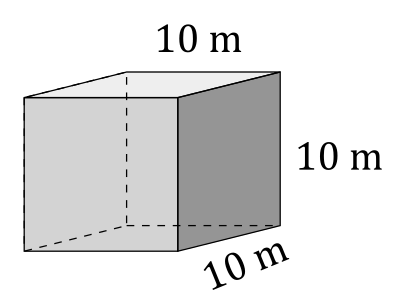
\includegraphics[width=10cm]{cube_tech_ill.png}
	
	\vfill


	{\large \today}
	 
	\end{center}

 \end{titlepage}


\chapter*{Learning outcomes}

\noindent The reader will learn:\\[0.4cm]

\noindent{\bf How to use it:}
\begin{itemize}
\item Basic GUI commands related to viewing the geometry
\item How to import CAD files into GMSH
\item How to generate basic stl and mesh files using gmsh
\item Basic commands for modifying the mesh resolution
\end{itemize}

\chapter*{Prerequisites}
\noindent The reader should know how to load/open ".geo" files into gmsh\\[0.4cm]
\tableofcontents


\chapter{Introduction}
This chapter introduces the associated files and importing features of GMSH.

\section{Associated Files}
Several files have been included along with this pdf. One of those files is a CAD file labelled "cube.iges" It consists of a set of curves and points that form a simple 10x10x10 meter cube.
\begin{figure}[h]
  \centering
  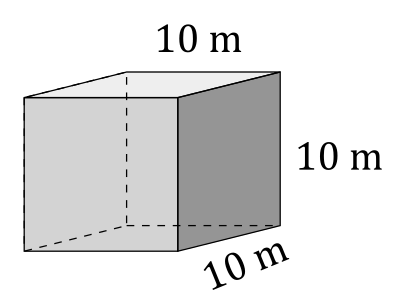
\includegraphics[width=10cm]{cube_tech_ill.png}
  \setcaptionwidth{10cm}
  \caption{Technical Illustration of the cube.iges file}
  \label{cube_tech_ill}
\end{figure}
Along with this iges file, there should also be several *.geo files. These files are the starting point for the tutorials in this pdf, all of which load the cube.iges CAD geometry. 

\newpage
\section{Importing and Viewing the Geometry}
A "cube0.geo" file is attached with this tutorial. Within that document are some basic importing commands. Note that any line that starts with "//" is a comment, simply there to describe the following command for the reader. The cube0.geo file sets some default OpenCASCADE values and then imports the cube.iges file. Open this cube0.geo file in gmsh. After doing so, you should see a set of curves and points.

When gmsh merges the cube.iges files, it converts the CAD curves and points into a set of points and curves that can be accessed through various gmsh commands. If you want to view the curve and point labels: go to Tools\textrightarrow Options\textrightarrow Geometry \textrightarrow Visibility, then check the "Curve Labels" and "Point Labels" boxes.
\begin{figure}[h]
  \centering
  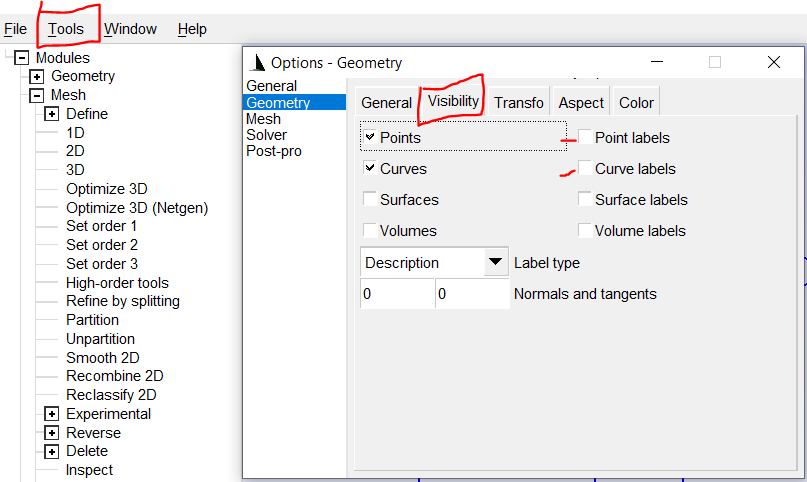
\includegraphics[width=7cm]{cube_visibility_options.png}
  \setcaptionwidth{8cm}
  \caption{Visibility Options}
  \label{cube_tech_ill}
\end{figure}

\begin{figure}[h]
  \centering
  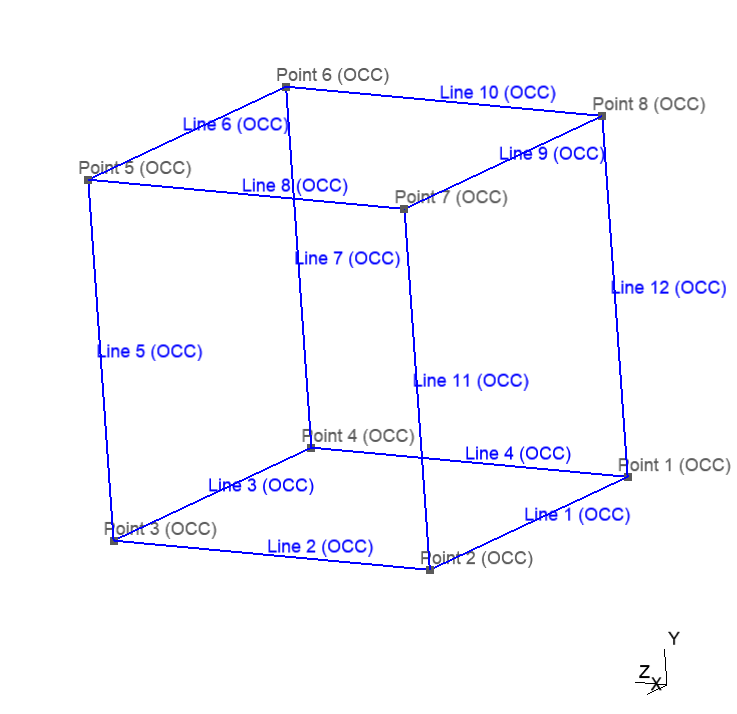
\includegraphics[width=10cm]{cube_points_curves.png}
  \setcaptionwidth{15cm}
  \caption{Labelled Curves and Points of the Entire Cube}
  \label{Cube_P_C}
\end{figure}
\newpage

Because this may be visually cluttering at times where you have more complex geometries, you may want to only look at a particular surface or set of surfaces. You can select to view a particular surface by going to Tools\textrightarrow Visibility, then clicking the surface you want to view, followed by clicking "Apply." After doing so, you should only see a single surface with it's curve and point labels.
\begin{figure}[h]
  \centering
  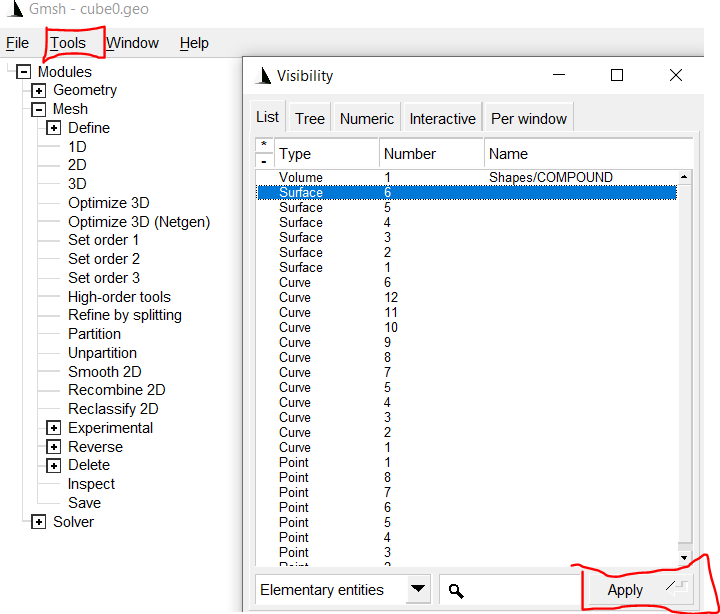
\includegraphics[width=7cm]{cube_visibility_options_2.png}
  \setcaptionwidth{7cm}
  \caption{Visibility Options for Single Surface}
  \label{cube_tech_ill}
\end{figure}

\begin{figure}[h]
  \centering
  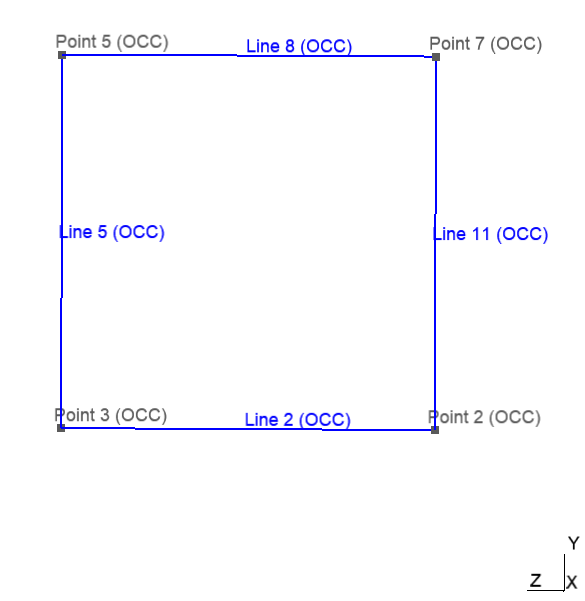
\includegraphics[width=8cm]{cube_1_surface.png}
  \setcaptionwidth{10cm}
  \caption{Labelled Curves and Points of a Single Surface}
  \label{Cube_P_C}
\end{figure}
 \newpage

\section{Viewing/Generating the Mesh}
Note that gmsh has a set of default meshing settings that are implemented whenever you open/create a new gmsh file. Because of these default settings, a mesh may be generated without specifying any meshing options. The mesh can be viewed in several ways, two of which are described here:
\begin{itemize}
\item If you are working with the gmsh GUI, you may simply click "2D" on the left-hand side to preview the surface mesh. The surface mesh can be saved through File\textrightarrow Export, and then choosing a file format (such as stl) and file name to export the mesh as.
\item If you instead want to use your terminal to generate the surface mesh file directly from the .geo file, you can type a command in your terminal such as: \begin{verbatim} gmsh cube0.geo -2 -o "cube.stl" -format stl \end{verbatim} 
\end{itemize}
If you get the error "command gmsh not found," you will need to configure your environment to locate the executable gmsh program (see the 00\_GMSH\_Introduction tutorial for instructions on how to set this up). The gmsh command above will take in the input geo file (gmsh cube0.geo), generate a 2D file (-2),  output the file name as "cube.stl" (-o "cube.stl"), and write the file contents specifically in the stl format (-format stl). The cube.stl file can then be opened in the gmsh GUI by File\textrightarrow Merge, then selecting the generated STL file. Otherwise, you may simply open the stl file in another visualization software such as paraview. The stl file should look similar to Figure \ref{Cube_defMesh}.

\begin{figure}[h]
  \centering
  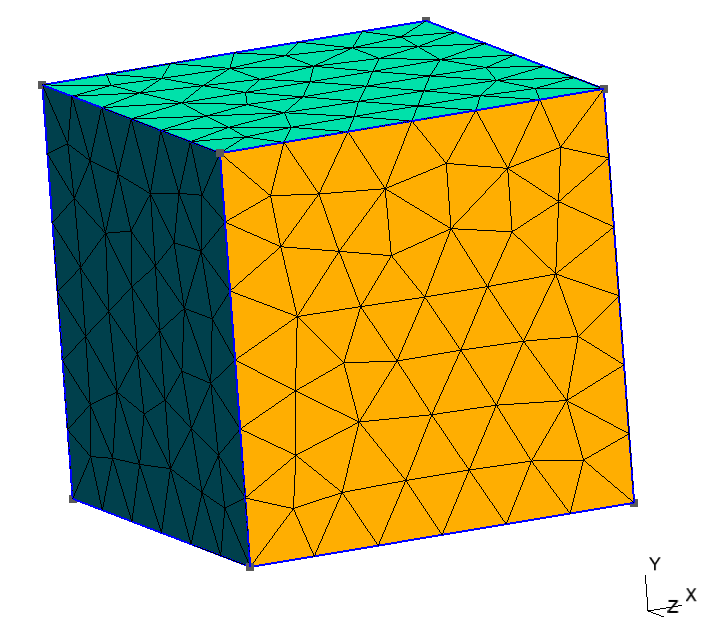
\includegraphics[width=8cm]{cube0_defaultMesh.png}
  \setcaptionwidth{10cm}
  \caption{STL File for a Cube using Default Mesh Settings for cube0.geo}
  \label{Cube_defMesh}
\end{figure}
 \newpage
\chapter{Modifying the Mesh Settings}
\section{Configuration}
This section describes how to add the gmsh pathway to your environment variables. \newline \newline
When you download the gmsh folder, you will see an gmsh.exe file located in the directory that you can double-click on to open gmsh. If you are trying to run gmsh from a windows terminal, you may also want to configure your environment so that the path of gmsh is known. (If you are unfamiliar with path and environment variables, see the documentation below). \newline \newline
https://superuser.com/questions/284342/what-are-path-and-other-environment-variables-and-how-can-i-set-or-use-them \newline \newline
Without specifying the path of gmsh, you would need to specify the path everytime you wanted to run gmsh from your terminal. For example, if my gmsh.exe file was located at: \begin{verbatim}
C:\Users\BarrDaniel\Downloads\gmsh-4.7.0-Windows64\gmsh-4.7.0-Windows64 \end{verbatim}  
, then I would need to type or copy/paste that entire pathway every single time that I wanted to run gmsh from my terminal. If you want to simply type ``gmsh'' in your terminal, you will need to edit your environment variables to include the pathway to this executable file. You can edit your pathway by searching for ``edit environment'' in the windows search box. \newline
\begin{figure}[h]
  \centering
  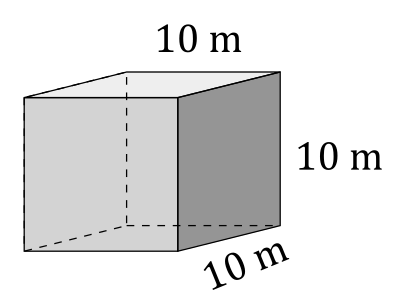
\includegraphics[width=15cm]{cube_tech_ill.png}
  \setcaptionwidth{15cm}
  \caption{Edit Environment Variables: Step 1}
  \label{TSDA_connected_bodies}
\end{figure}

\noindent (See images on next page for visualization of next steps) Click on ``Path'', then ``Edit'' to edit and add a new path. After this, you can add a new path by clicking on New, then pasting the pathway to your gmsh.exe file. Click ``OK'' then ``OK'' again in the next dialog box, and now your gmsh.exe should be added to your environment variables.

\newpage


\end{document}
